
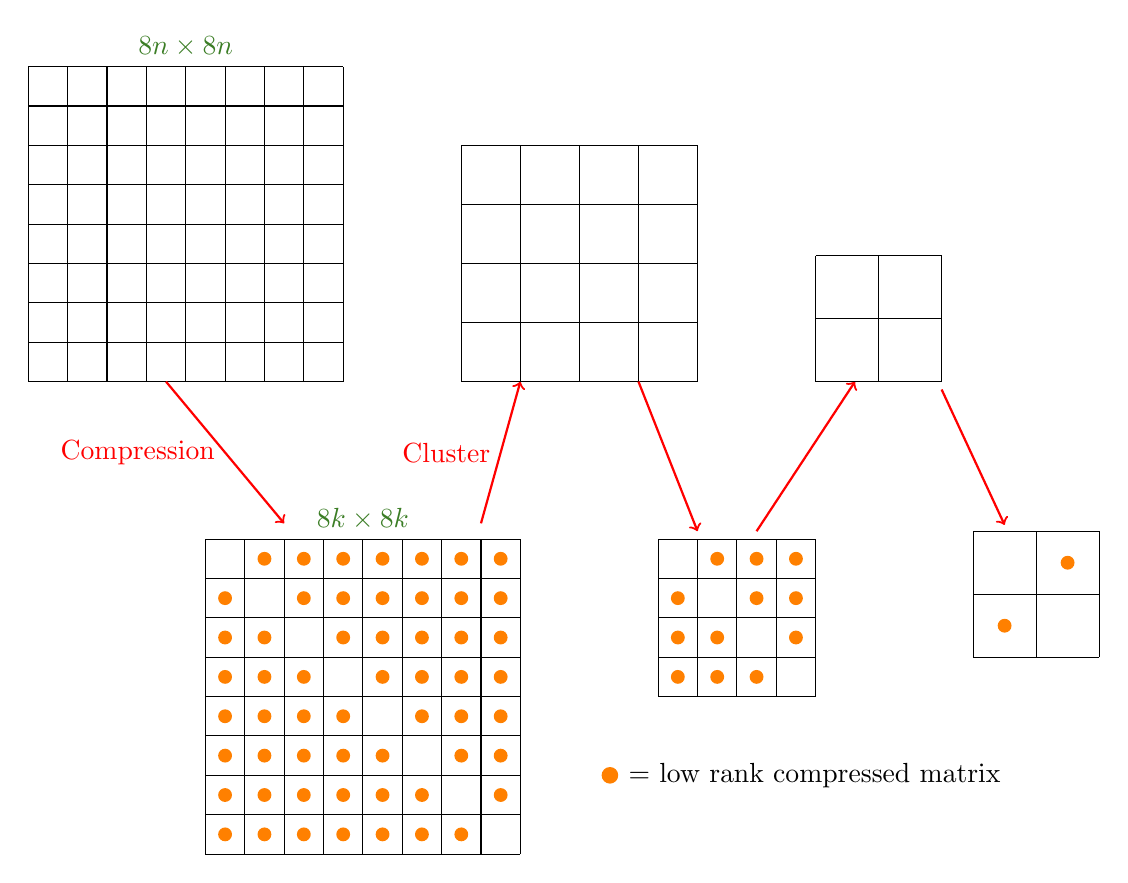
\begin{tikzpicture}

%% Step 1
\begin{scope}[]
    \draw[step=0.5] (0, 0) grid (4, 4);
    \node[OliveGreen]() at (2, 4.25){$8n\times 8n$};
\end{scope}

%% Step 2
\begin{scope}[
xshift = 2.25cm,
yshift = -6cm
]
    \draw[step=0.5] (0, 0) grid (4, 4);
    \node[OliveGreen]() at (2, 4.25){$8k\times 8k$};
    \draw[->, red, thick] (-0.5, 6) -- node[left]{Compression} (1, 4.2);
    \draw[->, red, thick] (3.5, 4.2) -- node[left]{Cluster} (4, 6);

    \foreach \i in {0.25, .75, ..., 3.75}{
        \foreach \j in {0.25, 0.75, ..., 3.75}{
        \node[inner sep=0pt, minimum size=5pt, fill, orange, circle]  () at (\i, \j) {};
        };
    };

    \foreach \i/\j in {
0.25/3.75,
0.75/3.25,
1.25/2.75,
1.75/2.25,
2.25/1.75,
2.75/1.25,
3.25/0.75,
3.75/0.25
    }{
        \node[inner sep=0pt, minimum size=6pt, fill, white]  () at (\i, \j) {};
    };
\end{scope}

%% Step 3
\begin{scope}[
xshift = 5.5cm,
scale=0.75
]
    \draw[step=1] (0, 0) grid (4, 4);
\end{scope}

%% Step 4
\begin{scope}[
xshift = 8cm,
yshift = -4cm,
scale=0.5
]
    \draw[step=1] (0, 0) grid (4, 4);
    \draw[->, red, thick] (-0.5, 8) -- (1, 4.2);
    \draw[->, red, thick] (2.5, 4.2) -- (5, 8);
    \foreach \i in {0.5, 1.5, ..., 3.75}{
        \foreach \j in {0.5, 1.5, ..., 3.75}{
        \node[inner sep=0pt, minimum size=5pt, fill, orange, circle]  () at (\i, \j) {};
        };
    };

    \foreach \i/\j in {
0.5/3.5,
1.5/2.5,
2.5/1.5,
3.5/0.5
    }{
        \node[inner sep=0pt, minimum size=6pt, fill, white]  () at (\i, \j) {};
    };
\end{scope}


%% Step 5
\begin{scope}[
xshift = 10cm,
scale=0.4
]
    \draw[step=2] (0, 0) grid (4, 4);
\end{scope}

%% Step 6
\begin{scope}[
xshift = 12cm,
yshift = -3.5cm,
scale=0.4
]
    \draw[step=2] (0, 0) grid (4, 4);
    \draw[->, red, thick] (-1, 8.5) -- (1, 4.2);
        \foreach \i in {1, 3, ..., 3.75}{
        \foreach \j in {1, 3, ..., 3.75}{
        \node[inner sep=0pt, minimum size=5pt, fill, orange, circle]  () at (\i, \j) {};
        };
    };
\foreach \i/\j in {
1/3, 3/1
    }{
        \node[inner sep=0pt, minimum size=6pt, fill, white]  () at (\i, \j) {};
    };
\end{scope}
\node[xshift=7.5cm, yshift=-5cm, right] () {= low rank compressed matrix};
\node[inner sep=0pt, left, minimum size=6pt, fill, orange, circle]  () at (7.5cm, -5cm) {};
\end{tikzpicture}
